\documentclass[../../tc_tp5_main.tex]{subfiles}

\begin{document}

%capítulo
\chapter{Celda Sallen-Key}

En esta secci\'on, se implementar\'an dos filtros pasabajos haciendo uso de celdas Sallen-Key en cascada. Sobre los mismos, se analizar\'a su respuesta en frecuencia, impedancia de entrada e impedancia de salida, y la sensibilidad de los par\'ametros caracter\'isticos del filtro a desviaciones en los valores de los componentes que lo integran respecto de su valor nominal. \par

Para esto, haremos en primer lugar un an\'alisis te\'orico de las celdas Sallen-Key.


\section{Introducci\'on: la celda Sallen-Key}

La Sallen-Key es una celda que permite realizar un filtro de segundo orden utilizando s\'olo \textit{op amps}, resistencias y capacitores. Si bien normalmente con estos dos tipos de componentes pasivos s\'olo podr\'ian obtenerse polos reales, es decir $Q \leq \nicefrac{1}{2}$, el \textit{feedback} positivo introducido por el operacional permite obtener polos complejos conjugados, y por lo tanto una mayor selectividad. Como en este tipo de celdas existe un \'unico \textit{feedback} positivo, en general la sensibilidad del filtro a la dispersi\'on de los par\'ametros del operacional es menor, y a los valores de los componentes pasivos es mayor, respecto de otro tipo de celdas.\par  

\begin{figure}[H]
	\centering
	\begin{circuitikz}
  	\draw (0,0) node[op amp, yscale=-1] (opamp) {}
  		(opamp.-) -| (-1.5, -1.5) node[left] {$V^-$}
  		to [R = $R_3$, *-]  (-1.5, -3.5) node[ground] {}
  		
  		(-1.5, -1.5) to [R = $R_4$] (1.5, -1.5) 
  		to [short, -*] (1.5, 0) to [short, -o] (2, 0) node[right] {$V_{out}$}
  		(1.5,0) to [short] (opamp.out) 
  		
  		(opamp.+) to [short, -*] (-2.5, 0.5) node[above]{$V^+$}
  		to [generic, l=$Z_3$] (-2.5, -1.5) node[ground]{}
  		
		(-2.5, 0.5) to [generic, l=$Z_2$] (-4.5, 0.5)
		to [generic, l=$Z_1$, *-o] (-6.5, 0.5) node[left]{$V_{in}$}  		
		
		(-4.5, 0.5) to [short, -*] (-4.5, 2) node[above] {$V_f$}
		to [generic, l=$Z_4$] (1.5,2)
		to [short] (1.5,0)
  	;
	\end{circuitikz}
	\caption{Celda Sallen-Key gen\'erica}
\end{figure}

En esta configuraci\'on, las resistencias $R_3$ y $R_4$ determinan la ganancia de la celda, puesto que forman un circuito no inversor en el camino del \textit{feedback} negativo. Las dem\'as impedancias, por otro lado, s\'olo tienen injerecia en la ubicaci\'on de los polos y los ceros del circuito, si bien la misma tembi\'en se ve afectada por las resistencias del no inversor.\par

Las ecuaciones que describen a este circuito son: 

\begin{equation}
	\left\{
 	\begin{aligned}
 		V_{out} &= A_{vol} \cdot (V^+ - V^-) \\
 		V^+ &= \frac{Z_2}{Z_2+Z_3} V_f  \\
		V^- &= \frac{R_3}{R_3+R_4} V_{out} \\
		\frac{V_{in} - V_f}{Z_1} &= \frac{V_f - V^+}{Z_2} +\frac{V_f - V_{out}}{Z_4} 
	\end{aligned}
	\right.
 \end{equation}
 
De esta \'ultima ecuaci\'on y expresando $V_f$ como funci\'on de $V^+$ se puede obtener que:

\begin{equation}
	V^+ = \left[ \left(1 + \frac{Z_3}{Z_2}\right) \cdot \left( \frac{1}{Z_1} + \frac{1}{Z_2} + \frac{1}{Z_4}\right) - \frac{1}{Z_2}\right] \cdot
			\left( \frac{V_{in}}{Z_1} + \frac{V_{out}}{Z_4}\right) = \frac{d}{Z_1} V_{in} + \frac{\gamma}{Z_4} V_{out}
\end{equation}

Por simplicidad, se efectu\'o la sustituci\'on $\gamma = \left(1 + \frac{Z_3}{Z_2}\right) \cdot \left( \frac{1}{Z_1} + \frac{1}{Z_2} + \frac{1}{Z_4}\right) - \frac{1}{Z_2}$.
Si llamamos adem\'as $K = 1 + \nicefrac{R_4}{R_3}$ a la ganancia del no inversor, esto se puede expresar mediante el siguiente diagrama de flujo de se\~nal: \par

\begin{figure}[H]
	\centering
	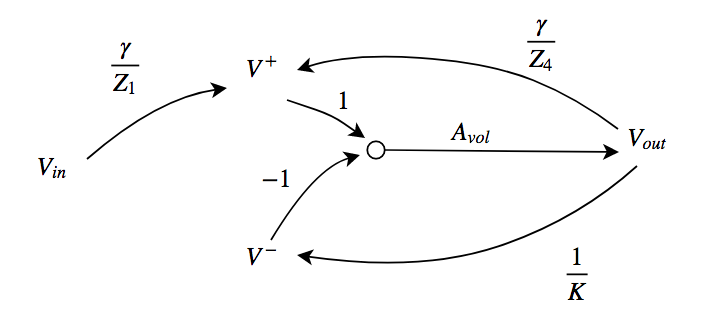
\includegraphics[scale=0.7]{imagenes/tc_tp1_ej1_df_1.png}
	
	\caption{Diagrama de flujo de se\~nal del circuito}
\end{figure}

Sucesivas simplificaciones permiten llevar el diagrama anterior a una forma que nos permita ver claramente los \textit{loops} de \textit{feedback} del circuito

\begin{figure}[H]
	\centering
	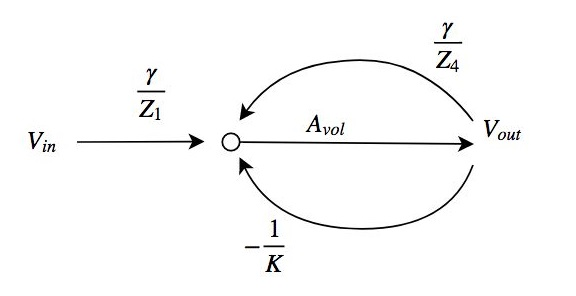
\includegraphics[scale=0.7]{imagenes/tc_tp1_ej1_df_2.jpg}\\
	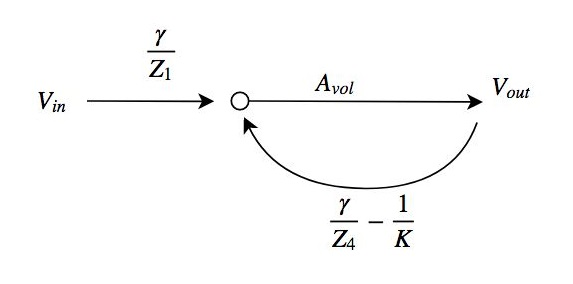
\includegraphics[scale=0.7]{imagenes/tc_tp1_ej1_df_3.jpg}	
	\caption{Simplificaciones del diagrama de flujo de se\~nal}
	\label{fig:1-flujo-de-senal}
\end{figure}

Partiendo de la figura \ref{fig:1-flujo-de-senal}, se puede obtener trivialmente la transferencia como:

\begin{equation}
	\frac{V_{out}}{V_{in}} = \frac{\gamma}{Z_1} \cdot \left( \frac{A_{vol}}{1 + A_{vol} \cdot \left( \frac{\gamma}{Z_4} - \frac{1}{K} \right)} \right)
	\label{eq:1-tf-sk-generica-avol}
\end{equation}

Si consideramos el caso ideal $A_{vol} \to \infty$, volviendo a reemplazar por el valor original de $\gamma$ obtenemos que:

\begin{equation}
	\frac{V_{out}}{V_{in}} = \frac{K}{ \frac{Z_1 Z_2}{Z_3 Z_4} + \frac{Z_1}{Z_3} + \frac{Z_2}{Z_3} + \frac{Z_1 \cdot (1-K)}{Z_4} + 1} 
	\label{eq:1-tf-sk-generica}
\end{equation}

En el caso particular de la celda Sallen-Key pasabajos, las sustituciones que se realizan son:

\begin{equation*}
	\left\{
 	\begin{aligned}
		Z_1 &=  R_1 & Z_3 &= \frac{1}{sC_2}\\
		Z_2 &= R_2 & Z_4 &= \frac{1}{sC_1}\\
	\end{aligned}
	\right.
 \end{equation*}


\begin{figure}[H]
	\centering
	\begin{circuitikz}
  	\draw (0,0) node[op amp, yscale=-1] (opamp) {}
  		(opamp.-) -| (-1.5, -1.5) 
  		to [R = $R_3$, *-]  (-1.5, -3.5) node[ground] {}
  		
  		(-1.5, -1.5) to [R = $R_4$] (1.5, -1.5) 
  		to [short, -*] (1.5, 0) to [short, -o] (2, 0) node[right] {$V_{out}$}
  		(1.5,0) to [short] (opamp.out) 	
  		
  		(opamp.+) to [short, -*] (-2.5, 0.5)
  		to [C, l_=$C_2$] (-2.5, -1.5) node[ground]{}
  		
		(-2.5, 0.5) to [R, l_=$R_2$] (-4.5, 0.5)
		to [R, l_=$R_1$, *-o] (-6.5, 0.5) node[left]{$V_{in}$}  		
		
		(-4.5, 0.5) to [short] (-4.5, 2)
		to [C, l=$C_1$] (1.5,2)
		to [short] (1.5,0)
  	;
	\end{circuitikz}
	\caption{Celda Sallen-Key pasabajos}
\end{figure}

 
Reemplazando en la ecuaci\'on \ref{eq:1-tf-sk-generica}, se obtiene que:

\begin{equation}
	\frac{V_{out}}{V_{in}} = \frac{K}{ s^2 \cdot R_1 R_2 C_1 C_2 + s \cdot \left[ R_1 (1-K) C_1 + (R_1 + R_2) C_2 \right] + 1}
\end{equation}

Efectivamente, esta ecuaci\'on corresponde a un filtro pasabajos de segundo orden, cuyos par\'ametros caracter\'isticos son:

\begin{equation}
	\left\{
 	\begin{aligned}
		f_0 &= \frac{1}{2\pi} \cdot \sqrt{\frac{1}{ R_1 R_2 C_1 C_2 }}\\
		Q &= \frac{\sqrt{ R_1 R_2 C_1 C_2 }}{  (R_1 (1-K) C_1 + (R_1 + R_2) C_2 }\\	
		G &= 1 + \frac{R_4}{R_3} 	
	\end{aligned}
	\right.
 \end{equation}
 
Como se ver\'a m\'as adelante, los dos filtros implementados con estas celdas tienen ganancia unitaria. Si bien podr\'ian utilizarse ganancias distintas de 1 en cada etapa, y si fuese necesario compensarlo con una etapa inversora o no inversora, por simplicidad s\'olo se considerar\'a el caso K = 1. Un posible problema de utilizar este criterio es que obtener un valor elevado de Q puede tornarse m\'as dif\'icil, o simplemente imposible, dadas las restricciones pr\'acticas a la hora de determinar los valores de los componentes. Sin embargo cabe destacar tambi\'en que si $K>1$, se debe prestar particular atenci\'on a no llegar a valores negativos para el coeficiente lineal del denominador de la transferencia, puesto que esto har\'ia que el sistema pierda su estabilidad, y por lo tanto as\'i nos desentendemos de este problema. \par

Para obtener ganancia unitaria, entonces, se reemplaza la resistencia $R_4$ por un cable y se deja un circuito abierto donde estar\'ia $R_3$, de forma tal que $G = 1 + \frac{R_4}{R_3} = 1$.
 
\begin{figure}[H]
	\centering
	\begin{circuitikz}
  	\draw (0,0) node[op amp, yscale=-1] (opamp) {}
  		(opamp.-) -| (-1.5, -1.5) 
		 to [short] (1.5, -1.5) 
  		to [short, -*] (1.5, 0) to [short, -o] (2, 0) node[right] {$V_{out}$}
  		(1.5,0) to [short] (opamp.out) 

  		(opamp.+) to [short, -*] (-2.5, 0.5)
  		to [C, l_=$C_2$] (-2.5, -1.5) node[ground]{}
  		
		(-2.5, 0.5) to [R, l_=$R_2$] (-4.5, 0.5)
		to [R, l_=$R_1$, *-o] (-6.5, 0.5) node[left]{$V_{in}$}  		
		
		(-4.5, 0.5) to [short] (-4.5, 2)
		to [C, l=$C_1$] (1.5,2)
		to [short] (1.5,0)
  	;
	\end{circuitikz}
	\caption{Celda Sallen-Key pasabajos con ganancia unitaria}
\end{figure}

<<<<<<< HEAD
Con esta configuraci\'on, las expresiones finales de $Q$ y $f_0$ son:

\begin{equation}
	\left\{
 	\begin{aligned}
		f_0 &= \frac{1}{2\pi} \cdot \sqrt{\frac{1}{ R_1 R_2 C_1 C_2 }}\\
		Q &= \frac{\sqrt{ R_1 R_2 C_1 }}{  (R_1 + R_2) \sqrt{C_2} }\\	
		G &= 1 
	\end{aligned}
	\right.
	\label{eq:f0-q}
 \end{equation}



\subsection{An\'alisis de sensibilidades} 

Antes de determinar los valores de los componentes que se utilizar\'an para cada filtro, estudiaremos a qu\'e componentes es m\'as sensible cada par\'ametro del circuito. A partir de las expresiones obtenidas en \ref{eq:f0-q}, utilizando la f\'ormula $S_x^y = \frac{x}{y} \cdot \frac{\partial y}{\partial x}$, se calcularon las sensibilidades relativas de $f_0$ y $Q$ a peque\~nas variaciones en los valores de los componentes que las integran.

\begin{table}[H]
	\centering
	\begin{tabular}{|c||c|c|c|c|}
	\hline
      	& $R_1$                                       & $R_2$                                     & $C_1$              & $C_2$              \\ \hline \hline
	$f_0$ & $-\nicefrac{1}{2}$                          & $-\nicefrac{1}{2}$                        & $-\nicefrac{1}{2}$ & $-\nicefrac{1}{2}$ \\ \hline
	$Q$   & $ - \frac{R_1 - R_2}{2 \cdot (R_1 + R_2)} $ & $ \frac{R_1 - R_2}{2 \cdot (R_1 + R_2)} $ & $\nicefrac{1}{2}$ & $\nicefrac{1}{2}$  \\ \hline
	\end{tabular}
	
	\caption{Sensibilidades de $f_0$ y $Q$ a los valores de los componentes}
\end{table}

Seg\'un estos resultados, la frecuencia del polo de una celda Sallen-Key de ganancia unitaria tiene la misma sensibilidad respecto de cada componente. En cuanto al factor de calidad, por otro lado, la sensibilidad a los capacitores es siempre $\pm \nicefrac{1}{2}$, pero a las resistencias depende de los valores de las mismas. Al igual que ocurr\'ia antes, $Q$ ser\'a siempre igual de sensible a ambas resistencias, aunque en este caso con signo opuesto, pero ahora si $R_1 = R_2$, esta sensibilidad es 0. Cuanto m\'as cercanos sean los valores de $R_1$ y $R_2$ entre s\'i, y m\'as grandes sean estos valores, menos sensible ser\'a $Q$ a estos par\'ametros. \par 

Por lo tanto, se tomar\'a el criterio de trabajar con resistencias iguales o cercanas entre s\'i, y siempre en el orden de los $k\Omega$. De esta manera, la sensibilidad de $Q$ a las resistencias no deber\'ia ser demasiado elevado. Por ejemplo, si se tomase en una celda $R_1 = 1k\Omega$ y $R_3 = 3k\Omega$, se tendr\'ia que $S_R^Q = \pm 0.5$, es decir que ser\'ia id\'entica a $S_C^Q$.\par 

Por otro lado, como todas las sensibilidades de $f_0$son $-0.5$ y no se cont\'o con la posibilidad de utilizar capacitores de tolerancias inferiores al $10\%$ para todos los valores, sabemos a priori que cada capacitor podr\'ia introducir un cambio de $-0.5 \cdot(\pm 10\%) = \mp5\%$ en el valor de $f_0$. Como hay dos capacitores por celda, esta dispersi\'on asciende a $10\%$. Por lo tanto, se determin\'o utilizar resistencias de tolerancia $1\%$, ya que de usar $5\%$ los cambios en los par\'ametros caracter\'isticos del circuito podr\'ian ascender al $15\%$, mientras que de esta manera se logra limitar este valor a $11\%$.


\section{Filtro 1: Legendre}

En primer lugar, se busca implementar un filtro pasabajos que cumpla la siguiente plantilla:

\begin{table}[H]
	\centering
	\begin{tabular}{|c|c|c|c|}
	\hline	
	Orden & $f_p$   & $A_p$ & $\abs{Z_{in}(f)}$           \\ \hline
	5     & $33kHz$ & $3dB$ & $\geq 50k\Omega\, \forall f$ \\ \hline
	\end{tabular}
	\caption{Plantilla del filtro pasabajos con Legendre}
\end{table}

Como no se tiene restricciones de $A_a$, se determin\'o utilizar $A_p' = 1$ a la hora de calcular la transferencia, de forma tal que la tolerancia de los valores de los componentes no provoque que no se cumpla la plantilla.\par

Habiendo obtenido la funci\'on transferencia de este filtro mediante la aproximaci\'on de Legendre, poniendo adem\'as la condici\'on de que todas las etapas deben tener ganancia unitaria, las etapas que se deben dise\~nar son las siguientes:

\begin{table}[H]
	\centering
	\begin{tabular}{|c||c|c|c|}
	\hline
	Etapa & Orden & $f_0\, (kHz)$ & Q    \\ \hline \hline
	1     & 1     & 29.5          & -    \\ \hline
	2     & 2     & 34.2          & 0.72 \\ \hline
	3     & 2     & 40.3          & 2.23 \\ \hline
	\end{tabular}
	\caption{Etapas del filtro 1}
\end{table}

\section{Filtro 2: Bessel}


=======

http://www.ti.com/lit/an/sloa024b/sloa024b.pdf
>>>>>>> parent of 266f140... codigo para histogramas pasabajos

\end{document}
